\section{Background}

The subsequent section presents background knowledge regarding different concepts and notions that will be adopted throughout the dissertation.
First, a definition of orientation frames and coordinate systems will be presented, followed by an introduction to Euler angles and quaternions, building a foundation of understanding wherein the mathematics and arithmetic behind attitude representation. An introduction to inertial sensors and how they can be employed to estimate orientation is then exhibited. The chapter concludes with an analysis and summary of different sensor fusion algorithms utilized to determine orientation.

\subsection{Frames of coordinates}

This section will focus on defining and distinguishing the different concepts of frame coordinate systems. An emphasis will be given to East North Up (ENU), Earth Centered, Earth Fixed (ECEF), and the World Geodetic System (WGS84). The notion of body frame will also be defined. The ECEF and WGS84 can be considered supplementary frame systems applied to describe the ENU frame, which can be understood as the world frame.

\subsubsection{ECEF and ENU frame}

ECEF coordinate system describes a referential axis where the origin of the coordinates is at the center of mass of the Earth, also known as barycenter. Mathematically, this translates to the integral of the position vector times the density over the Earth being zero (equation \ref{eqn:ecef}).

\begin{equation}
    \int \overrightarrow{x}\rho~dx^3 = 0
    \label{eqn:ecef}
\end{equation}

The X-axis is described by the intersection of the zero-latitude line (Equator) plan and the zero-longitude line (prime meridian) plan. The orientation of the X-axis is deemed to be positive from the center towards the point defined by zero latitude and longitude. Z-axis is expressed by the line interconnecting North and South Poles, staying positive in the Earth’s barycenter to the North Pole. Y-axis lies in the equatorial plane and is perpendicular to the plane described by the X and Z-axis, and it is in a positive direction.  The right-hand rule explains its orientation.

The East North Up (ENU) system is a geographic coordinate structure where the origin is placed at an empirical point in the ECEF coordinate system.  In the ENU coordinate system, the X-axis points towards the East, and the Y-axis aims over the North Pole. The plane described by the X and Y-axis is tangential to the WGS84 frame on the origin of ENU. Z-axis designates the elevation from a defined geographical plane (figure \ref{fig:ECEF}). The ENU frame is considered in this work as the reference frame.

\begin{figure}[H]
    \centering
    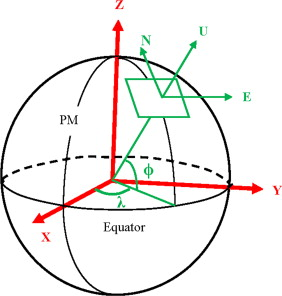
\includegraphics[width=0.5\textwidth]{figures/ECEF.jpg}
    \caption{An illustrative diagram for the WGS84, ECEF, and ENU coordinate systems for the Earth and their transformation correlation (PM line is the Prime Meridian; $\phi$ and $\lambda$ are latitude and longitude in WGS84; X, Y, Z for ECEF; and E, N, U for ENU).  }
    \label{fig:ECEF}
\end{figure}

Considering a point of reference in the ECEF frame, it is required to discover the equivalent latitude and longitude of the reference point (Xr, Yr, Zr). The parameters of WGS84 required to perform such transformation are presented in table \ref{tab:WGS}.

\begin{table}[H]
    \begin{center}
        \begin{tabular}[t]{lcc}
            \hline
            Parameter                   & Notation & Value                 \\
            \hline
            Semi-major axis             & $a$      & 6 378 137.0 m
            \\
            Reciprocal of flattening    & $1/f$    & 298.257 223 563
            \\
            Semi-minor axis             & $b$      & 6 356 752.3142 m      \\
            First eccentricity squared  & $e^2$    & 6.694 379 990 14x10-3 \\
            Second eccentricity squared & $e'^{2}$ & 6.739 496 742 28x10-3 \\
            \hline
        \end{tabular}
        \caption{WGS 84 needed parameters to convert ECEF coordinates into ENU. }
        \label{tab:WGS}
    \end{center}
\end{table}

Applying the set of equations (\ref{eq:transformation}) to approximate latitude ($\psi_r$) and longitude ($\phi_r$) for the reference coordinate point. The last transformation outcome in applying equation (\ref{eq:transformation_results}) to ECEF physical quantities.

\begin{equation}
    \begin{aligned}
         & p = \sqrt{(X_r)^2 + (Y_r)^2}                                                      \\
         & \theta = \arctan(Z_r\frac{a}{pb} )                                                \\
         & \lambda_r = \arctan(Y_r,X_r)                                                      \\
         & \varphi_r = \arctan(\frac{Z_r + e^2 b\sin^3(\theta)}{p - e^2 a \cos^3(\theta )} ) \\
    \end{aligned}
    \label{eq:transformation}
\end{equation}

\begin{equation}
    \begin{bmatrix}
        x \\
        y \\
        z
    \end{bmatrix}_{ENU}
    =
    \begin{bmatrix}
        -\sin(\lambda_r)             & \cos( \phi_r)                  & 0            \\
        -\sin(\phi_r)\cos(\lambda_r) & -\sin( \phi_r)\sin(\lambda_r)  & \cos(\phi_r) \\
        \cos(\phi_r)\cos(\lambda_r)  & \cos( \phi_r)  \sin(\lambda_r) & \sin(\phi_r)
    \end{bmatrix}
    \begin{bmatrix}
        X_p - X_r \\
        Y_p - Y_r \\
        Z_p - Z_r
    \end{bmatrix}_{ECEF}
    \label{eq:transformation_results}
\end{equation}

\subsubsection{Body frame}

Each sensor present in the razor board is aligned to match the sensor axes printed in the board as seen in figure 3.1. For simplicity, the razor sensors are placed as possible near the middle point of the bisector segment between the two wheel axes in such a away that YY axis as marked in the figure 3.1 is pointing towards the front of vehicle, XX axis is pointing to the right side of the car and ZZ axis is pointing to the top. This way, if the Euler angles describing the orientation of body frame related to world frame are all equal to zero, it means the axes in each frame are coincident apart from an offset in origin. Rotation angles are considered positive following the right hand rule in each axis. The origin of body frame is equal to intersection of rear wheel axis with the bisector defined above.

\subsection{Orientation}

The attitude orientation of a UAV is a critical aspect in autonomous flight. In a low-cost
AHRS, accuracy and low complexity are important in calculating the attitude of the UAV.
There are various ways to represent attitude including: rotational matrices, Euler angles and quaternions.

\subsubsection{Rotation Matrix}

The rotation matrix is a concept employed to express the transformation of coordinates from one frame to another. In addition, it can also convey orientation of one frame relative to another. Any orientation can be attained by composing three elemental rotations, beginning from a known standard orientation. Analogously, any rotation matrix R can be decomposed as a product of three elemental rotation matrices (equation \ref{eq:rotation_matrices}).

\begin{equation}
    R = X(\alpha)Y(\beta)Z(\gamma)
    \label{eq:rotation_matrices}
\end{equation}

In equation \ref{eq:rotation_matrices}, $R$ is a rotation matrix that can be applied to represent a composition of intrinsic rotations about axes $X$, $Y$, $Z$, (in that order), or a composition of extrinsic rotations about axes $Z$, $Y$, $X$ (in that order). The convention used in this work is represented by equation \ref{eq:axes_frames} and maps quantities described in frame $b$ to frame $a$. Comparing the structure of (2.3) with figure \ref{fig:axes_frames} it is seen that columns of $^a_bR$ represent each unity vector defining all axes of frame $b$.


\begin{figure}[!h]
    \centering
    \resizebox{0.49\linewidth}{!}{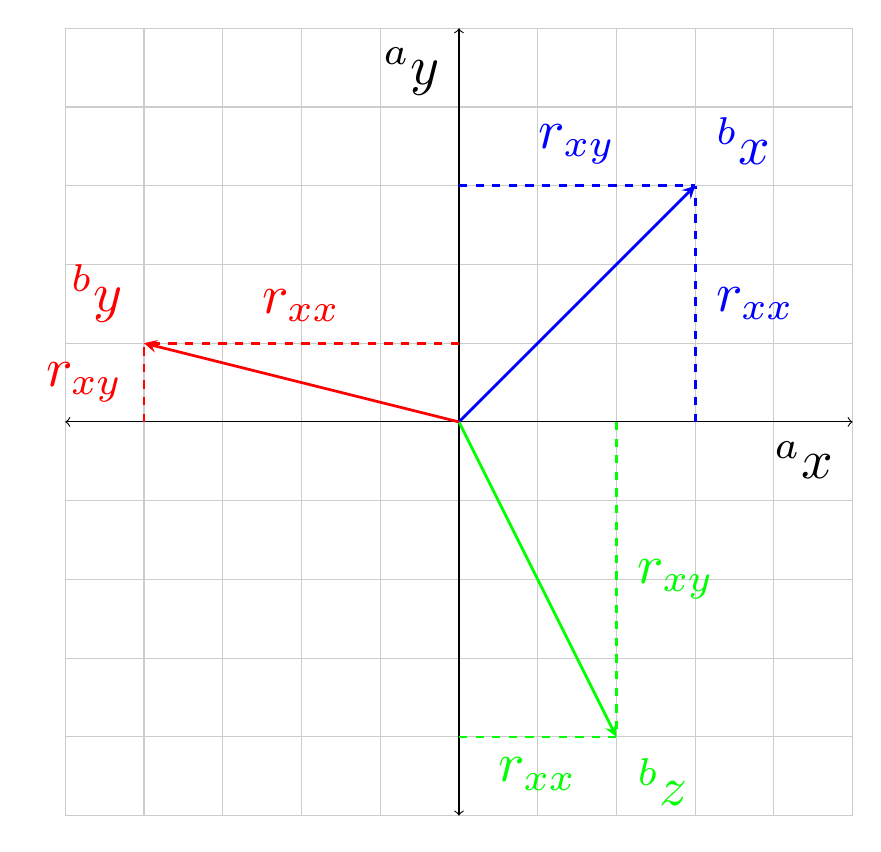
\begin{tikzpicture}
    \draw[thin,gray!40] (-5,-5) grid (5,5);
    \draw[<->] (-5,0)--(5,0) node[anchor=north east, scale=2]{$^{a}x$};
    \draw[<->] (0,-5)--(0,5) node[anchor=north east, scale=2]{$^{a}y$};
    \draw[line width=1pt,blue,-stealth](0,0)--(3,3) node[anchor=south west, scale=2]{$^{b}x$};
    \draw[line width=1pt,blue,dashed](3,0)--(3,3) node[midway, right, scale=2]{$r_{xx}$};
    \draw[line width=1pt,blue,dashed](0,3)--(3,3) node[midway, above, scale=2]{$r_{xy}$};
    \draw[line width=1pt,green,-stealth](0,0)--(2,-4) node[anchor=north west, scale=2]{${^{b}z}$};
    \draw[line width=1pt,green,dashed](0,-4)--(2,-4) node[midway, below, scale=2]{$r_{xx}$};
    \draw[line width=1pt,green,dashed](2,0)--(2,-4) node[midway, right, scale=2]{$r_{xy}$};
    \draw[line width=1pt,red,-stealth](0,0)--(-4,1) node[anchor=south east, scale=2]{${^{b}y}$};
    \draw[line width=1pt,red,dashed](0,1)--(-4,1) node[midway, above, scale=2]{$r_{xx}$};
    \draw[line width=1pt,red,dashed](-4,0)--(-4,1) node[midway, left, scale=2]{$r_{xy}$};
\end{tikzpicture}}
    \resizebox{0.49\linewidth}{!}{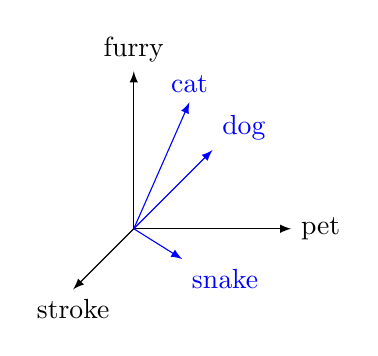
\begin{tikzpicture}
    % \draw[thin,gray!40] (-5,-5,0) grid (5,5,0);
    \draw[-latex] (0,0,0) -- (2,0,0)node[anchor=west]{pet};
    \draw[-latex] (0,0,0) -- (0,2,0)node[anchor=south]{furry};
    \draw[-latex] (0,0,0) -- (0,0,2)node[anchor=north]{stroke};
    \draw[blue,-latex] (0,0,0) -- (1,1,0)node[anchor=south west]{dog};
    \draw[blue,-latex] (0,0,0) -- (1,0,1)node[anchor=north west]{snake};
    \draw[blue,-latex] (0,0,0) -- (0.9,1.8,0.5)node[anchor=south]{cat};
\end{tikzpicture}}
    \caption{Sensor data on each axis (blue is X-axis, red is Y-axis, green is Z-axis) obtained by the accelerometer, gyroscope, and magnetometer at 100 Hz sampling rate. Accelerometer provided the system’s proper acceleration; gyroscope supplied the body’s angular rate, and the magnetometer presented the detected magnetic flux.}
    \label{fig:axes_frames}
\end{figure}


\begin{equation}
    \textrm{$_{b}^{a}R$}
    =
    \begin{bmatrix}
        \textrm{$^{a}r_{xx}$} & \textrm{$^{a}r_{yx}$} & \textrm{$^{a}r_{zx}$} \\
        \textrm{$^{a}r_{xy}$} & \textrm{$^{a}r_{yy}$} & \textrm{$^{a}r_{zy}$} \\
        \textrm{$^{a}r_{xz}$} & \textrm{$^{a}r_{yz}$} & \textrm{$^{a}r_{zz}$} \\
    \end{bmatrix}
    \label{eq:axes_frames}
\end{equation}

Rotation matrices belong to the orthonormal group and one important property is that bRa bRT = I meaning a bRT = a bR−1 . Also a bRT is equal to b aR [36][37].

\subsubsection{Euler angles}

Euler angles are a well-known form to represent attitude with respect to a fixed coordinate system. Mathematically, Euler angles represent three composed sequential rotations that stir a reference frame to a given referred frame. It expresses a rotation in three angles, often referred to as pitch, roll and yaw, denoted by $\phi$, $\theta$ and $\psi$. These angles represent three consecutive rotations about the axes of the coordinate frame, for example z-x-z 0: First rotate $\phi$ radians about the z-axis, then rotate $\theta$ radians about the x-axis and finally rotate $\psi$ radians about the new z-axis. According to differential equations of Euler angles givens (equation \ref{eq:euler_equation}), $\phi$, $\theta$, and $\psi$ can be solved based on angular rate measurements. Only three differential equations need solving before the attitude gets clearly estimated. However, there exists a serious shortcoming with this solution. As cos $\theta$ approaches zero, the differential equations degrade fast and the solution becomes badly inaccurate, which means that these equations cannot give effective attitude solution at some singular points of the attitude space:


\begin{equation}
    \begin{bmatrix}
        \dot{\psi}   \\
        \dot{\theta} \\
        \dot{\phi}   \\
    \end{bmatrix}
    =
    \frac{1}{\cos(\phi)}
    \begin{bmatrix}
        \sin(\phi)             & 0 & -\cos(\phi)            \\
        \cos(\theta)\cos(\phi) & 0 & \cos(\theta)\sin(\phi) \\
        \sin(\theta)\sin(\phi) & 1 & \sin(\theta)\cos(\phi)
    \end{bmatrix}
    \begin{bmatrix}
        \omega{^b_{nbx}} \\
        \omega{^b_{nby}} \\
        \omega{^b_{nbz}} \\
    \end{bmatrix}
    \label{eq:euler_equation}
\end{equation}

The order of which the angles are represented in a vector is not important, however the
order of rotation is. The order of rotation used in the implemented Kalman filter algorithm is: roll, pitch, and yaw. The reason for using this ordering is due to how the attitude is perceived. A UAV in autonomous flight typically does not incline or decline at a high rate, however it may roll at a high rate. To accurately understand the orientation of the UAV with respect to the Euler angles, it must be read from the roll first, then pitch, then yaw.
The roll will have the range of ±180, this allows the pitch to have the range of ±90◦. The
yaw is represented using the range of ±180◦. The convention is used to keep the accurate
orientation of the plane.

Euler angles have one disadvantage, which is known as Gimbal lock. Euler angles act
as a gimballed system, where the three axes can be thought of as three separate gimbals
connected together. Gimbal lock occurs when two axis are aligned, such as when the plane
is pitched straight up, the pitch an the yaw axis are aligned, and as the roll gimbal is rotated, the pitch and the yaw angle are both effected the same, therefore losing orientation. The singularity problem can be fixed by adding another gimbal, or using an ad hoc approach to hard code values or use limits in the algorithm. The approach used in this thesis is to use a different representation adding another gimbal, known as quaternions. It is necessary to use an attitude representation with the least amount of elements because of the low-cost system requirements of low complexity. Whenever propagating attitude estimation through the Kalman filter, matrix multiplication increases in comlexity with more elements, especically in finding the inverse of a matrix.

\subsubsection{Quaternions}

As stated previously, to eliminate the singularities at ±90◦ on the pitch and roll axes, and
to keep the computational efficiency optimal, quaternions are used for state attitude representation. To understand quaternions, one must first understand the complex number
relationship. A complex number can represent a rotation in 2 dimensional coordinate frame
with a real x-axis and imaginary axis y-axis or vise versa.
A quaternion is the same concept, except instead of one imaginary axis, there are three
imaginary axes; in a sense its like combining three complex numbers into one. To go from a
2D interpretation to a 3D, four components are required; one real component qs and three
imaginary qx qy qz which can also be represented as a vector ˜v. Equation (2.1) shows this
relation with the complex number x having a real part a and imaginary part b; and the
quaternion q containing a real scalar part s and an imaginary vector component ~v.
To visualize a quaternion operation, think of Euler angles in the sense that there are
three orthogonal angles each on a separate mutually exclusive axis, x,y and z as shown in
figure 2.2. The rotation is not simultaneous, each rotation must happen sequentially, one
axis at a time. In navigation terms, the plane must roll, then pitch, then yaw. In quaternion
terms, the sequence can be thought of the same way as a rotating a vector laying on the
x-axis, then rotating a vector on the y-axis, and finally rotating a vector on the z-axis.

\begin{equation}
    q = q_1 + q_2 i + q_3 j + q_4 k
\end{equation}

\begin{equation}
    q =     \begin{bmatrix}
        q_1 &  & q_2 &  & q_3 &  & q_4 \\
    \end{bmatrix}
\end{equation}

\begin{equation}
    \hat{q} \Longrightarrow \left\lVert q\right\rVert =1
\end{equation}

\begin{equation}
    i^2=j^2=k^2=ijk=-1
\end{equation}

\begin{equation}
    ij = -j1 = k
\end{equation}

\begin{equation}
    ki = -ik = j
\end{equation}

\begin{equation}
    ki = -ik = j
\end{equation}

\begin{equation}
    a \otimes b = \left[a_1 a_2 a_3 a_4\right] \otimes \left[b_1 b_2 b_3 b_4\right]     =
    \begin{bmatrix}
        a_1 b_1 - a_2 b_1 - a_3 b_3 - a_4 b_4 \\
        a_1 b_2 + a_2 b_2 + a_3 b_4 - a_4 b_3 \\
        a_1 b_3 - a_2 b_3 + a_3 b_1 + a_4 b_4 \\
        a_1 b_4 + a_2 b_4 - a_3 b_2 + a_4 b_1 \\
    \end{bmatrix}
\end{equation}

\begin{equation}
    \textrm{$_{b}^{w}q$}^* =\textrm{$_{w}^{b}q$} = \left[q_1 - q_2 - q_3 - q_4\right]
\end{equation}

\begin{equation}
    \textrm{$^{b}v$} = \textrm{$_{b}^{w}\hat{q}$} \otimes \textrm{$^{w}v$} \otimes \textrm{$_{b}^{w}\hat{q}$}^*
\end{equation}

\begin{equation}
    \textrm{$_{c}^{a}\hat{q}$} = \textrm{$_{c}^{b}\hat{q}$} \otimes \textrm{$_{b}^{a}\hat{q}$}
\end{equation}

\subsubsection{Accelerometer}
\subsubsection{Gyroscope}
\subsubsection{Magnetometer}
\subsection{Sensor Fusion}
\subsubsection{Sensor Fusion Algoritms}
\paragraph{Kalman Filter}

The Kalman filter algorithm is a set of mathematical equations that provides a computationally efficient approach to estimate some unknown variables by the detected measurements\cite{welch1995introduction}. Kalman filters operate recursive functions to predict the present state of a linear problem by monitoring the current input data, the previous input data, and the previous state prediction.  Two generally assigned methods for Kalman filter-based sensor fusion are state-vector fusion and measurement fusion. The state-vector fusion method (figure \ref{fig:statekalman}) applies a group of Kalman filters to acquire individual sensor-based state estimates, which are subsequently fused to obtain an enhanced combined state estimate. Measurement fusion (figure \ref{fig:mesearurmentkalman}) approach directly combines the sensor data to achieve a joint measurement and later uses a single Kalman filter to get hold of the final state estimate centered on the fused measurement \cite{mosallaei2007process}.
When applied appropriately, Kalman filters offer highly precise orientation, even with the existence of substantial noise. Nevertheless, Kalman filters are computationally expensive rising hardware cost and latency. They are also of complex implementation, which, shared with computational overhead, can make the algorithm unfeasible for computationally restricted applications. They are regularly useful in a wide-ranging variety of applications and have become a standard method in sensor fusion. Several studies examine the possibility of using Kalman filters to predict a body’s orientation and position by combining multiple sensors. The Kalman filter is founded on recursive Bayesian filtering.
Consequently, the system’s noise is assumed to be Gaussian. Therefore, the Kalman filter is generally suggested for linear systems. For this reason, an extension of the classic Kalman Filter designed for non-linear systems has emerged, recognized as Extended Kalman filter \cite{wilson2019formulation}.


\begin{figure}
    \centering
    \begin{subfigure}[b]{0.45\textwidth}
        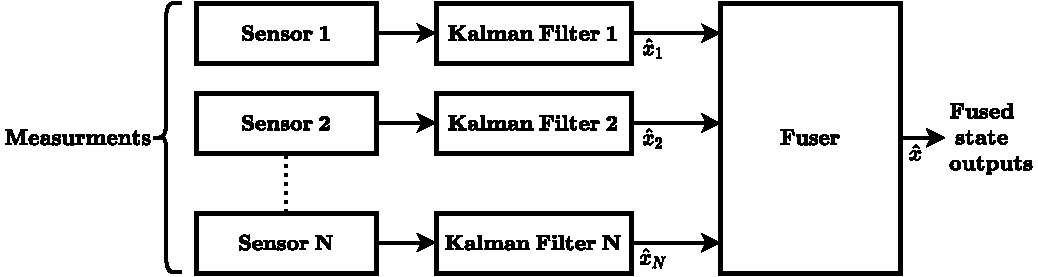
\includegraphics[width=1\linewidth]{figures/kalman1.pdf}
        \caption{}
        \label{fig:statekalman}
    \end{subfigure}
    \begin{subfigure}[b]{0.45\textwidth}
        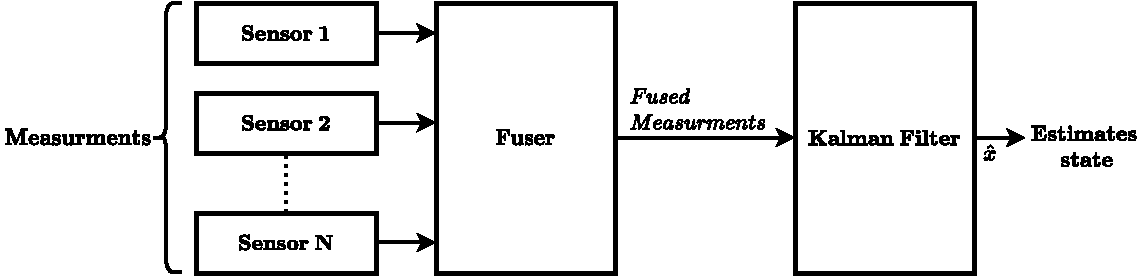
\includegraphics[width=1\linewidth]{figures/kalman2.pdf}
        \caption{}
        \label{fig:mesearurmentkalman}
    \end{subfigure}

    \caption{ Kalman-filter-based multi-sensor data fusion.
        (a) State-vector fusion. (b) Measurement fusion. \cite{mosallaei2007process} }
\end{figure}

\paragraph{Complementary Filter}

The complementary filter is considered a simpler approach relatively to the Kalman filter since it is a computationally lightweight solution and straightforward to implement \cite{higgins1975comparison}. This filter takes as input two noisy sensor measurements and assumes one input is mainly formed by high-frequency signals whereas the other is mostly by low-frequency signals. Through a low pass filter, the high-frequency noise of the first input is filtered out. An identical procedure occurs with the second signal, but this time with a high pass filter to remove low-frequency noises, as illustrated in figure \ref{fig:complementary}. Yet, the complementary filter is not especially robust to noisy or biased data since it simply uses currently available information, therefore, has no direct method of compensating for sensor noise \cite{wilson2019formulation}. A conventional application of the complementary filter is to bring together measurements of vertical acceleration and barometric readings to attain an approximation of vertical velocity. Similar to the Kalman filter, new versions built upon the principles of the classic complementary filter have emerged in recent times, such as the Extended Complementary Filter (ECF). They promise a high level of accuracy and enhanced robustness to noise while preserving computational efficiency.

\begin{figure}[!h]
    \centering
    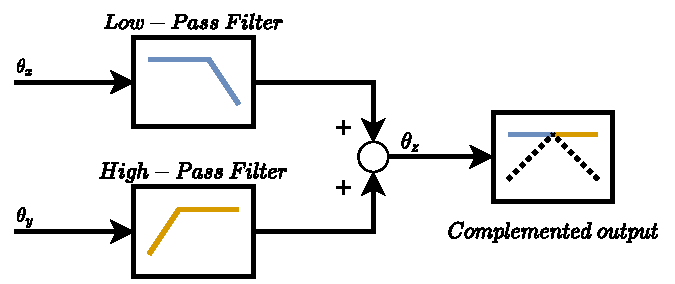
\includegraphics[width=0.7\textwidth]{figures/complementary.pdf}
    \caption{Basic complementary filter \cite{higgins1975comparison} - Two different measurement sources for estimating one variable. The noise properties of the two measurements are such that one source gives good information only in low frequency region while the other is good only in high frequency region. }
    \label{fig:complementary}
\end{figure}

\paragraph{Optimization Filters}

Up until recently, there remained mainly two distinct AHRS fusion approaches. One category including the complementary filters, and the other is related to Kalman filtering. Some recent AHRS algorithms have emerged in the literature over the past years. Two of the most prominent are the Mahony and Madgwick algorithms, which have been categorized as optimization filters. Optimization filters obtain orientation by assessing a vector representative of the sensor output at the present orientation and lessening the disparity concerning predicted and observed outputs. Optimization filters are well established for linking accuracy with computational expense and simplicity of implementation \cite{madgwick2020extended}.
Both methods make use of a quaternion representation, which is a four-dimensional complex number representing of an object orientation. Quaternions involve fewer computation time because of their minimal quantity of calculation parameters \cite{ludwig2018comparison}. Additionally, vector rotations are easily executed by quaternion multiplications.
Madgwick et al. \cite{madgwick2010efficient} pioneered a gradient descent fusion algorithm, frequently recognized as ‘Madgwick Algorithm.’ This gradient descent fusion algorithm first obtains a quaternion estimation of the gyroscope output integration and later corrects it with a quaternion from the accelerometer and magnetometer data. Madgwick’s approach guarantees decent attitude estimation at a low computational cost. Further, it tackles the difficulty of the local magnetic disturbances that can influence all the orientation components. By reducing the constraint of the magnetic field vector rotation, it can limit the effect of the magnetic disturbances to only affect the yaw component of the orientation.

\paragraph{Other Filters}
\subsection{Low-Cost Inertial Measurement Units}
\subsubsection{MPU-9150 Evaluation Board 9DOF}